\documentclass[openany]{book}

\usepackage[margin=1in]{geometry}
\usepackage{amsmath,amsfonts,amsthm}
\usepackage{xcolor}
\renewcommand{\familydefault}{ppl}
\newcommand{\E}{\mathbb{E}}
\newcommand{\F}{\mathbb{F}}
\newcommand{\R}{\mathbb{R}}
\newcommand{\Z}{\mathbb{Z}}
\newcommand{\la}{\langle}
\newcommand{\ra}{\rangle}
\newcommand{\colim}{\text{colim}}
\newcommand{\T}{\mathcal{T}}

\DeclareMathOperator{\im}{im}
% command+/

\usepackage{quiver}
\usepackage{tikz-cd}


\usepackage{thmtools,thm-restate}

% Fixing mdframed skip below
% See https://tex.stackexchange.com/a/292090/143086
\usepackage[framemethod=TikZ]{mdframed}
\usepackage{xpatch}
\makeatletter
\xpatchcmd{\endmdframed}
	{\aftergroup\endmdf@trivlist\color@endgroup}
	{\endmdf@trivlist\color@endgroup\@doendpe}
	{}{}
\makeatother

\definecolor{huilightpink}{HTML}{fcf2f9}
\definecolor{huidarkpink}{HTML}{ed34b3}
\declaretheoremstyle[
	mdframed={
		backgroundcolor=huilightpink,
		linecolor=huidarkpink,
		rightline=false,
		topline=false,
		bottomline=false,
		linewidth=2pt,
		innertopmargin=5pt,
		innerbottommargin=8pt,
		innerleftmargin=8pt,
		leftmargin=-2pt,
		skipbelow=2pt,
		nobreak
	},
	headfont=\normalfont\bfseries\color{huidarkpink}
]{huipinkbox}
\declaretheorem[style=huipinkbox,name=Theorem,within=chapter]{thm}
\declaretheorem[style=huipinkbox,name=Theorem,sibling=thm]{theorem}



\definecolor{huilightpurple}{HTML}{faf2ff}
\definecolor{huidarkpurple}{HTML}{912ed9}
\declaretheoremstyle[
	mdframed={
		backgroundcolor=huilightpurple,
		linecolor=huidarkpurple,
		rightline=false,
		topline=false,
		bottomline=false,
		linewidth=2pt,
		innertopmargin=5pt,
		innerbottommargin=8pt,
		innerleftmargin=8pt,
		leftmargin=-2pt,
		skipbelow=2pt,
		nobreak
	},
	headfont=\normalfont\bfseries\color{huidarkpurple}
]{huipurplebox}
\declaretheorem[style=huipurplebox,name=Proposition,within=chapter]{prop}

\definecolor{huilightpurple}{HTML}{faf2ff}
\definecolor{huidarkpurple}{HTML}{912ed9}
\declaretheoremstyle[
	mdframed={
		backgroundcolor=huilightpurple,
		linecolor=huidarkpurple,
		rightline=false,
		topline=false,
		bottomline=false,
		linewidth=2pt,
		innertopmargin=5pt,
		innerbottommargin=8pt,
		innerleftmargin=8pt,
		leftmargin=-2pt,
		skipbelow=2pt,
		nobreak
	},
	headfont=\normalfont\bfseries\color{huidarkpurple}
]{huipurplebox}
\declaretheorem[style=huipurplebox,name=Lemma,within=chapter]{lem}

\declaretheorem[style=huipurplebox,name=Corollary,within=chapter]{cor}


\definecolor{huilightblue}{HTML}{edf9ff}
\definecolor{huidarkblue}{HTML}{4b79db}
\declaretheoremstyle[
	mdframed={
		backgroundcolor=huilightblue,
		linecolor=huidarkblue,
		rightline=false,
		topline=false,
		bottomline=false,
		linewidth=2pt,
		innertopmargin=5pt,
		innerbottommargin=8pt,
		innerleftmargin=8pt,
		leftmargin=-2pt,
		skipbelow=2pt,
		nobreak
	},
	headfont=\normalfont\bfseries\color{huidarkblue}
]{huiblueblox}
\declaretheorem[style=huiblueblox,name=Definition,within=chapter]{defn}

\definecolor{huilightblue}{HTML}{edf9ff}
\definecolor{huidarkblue}{HTML}{4b79db}
\declaretheoremstyle[
	mdframed={
		backgroundcolor=huilightblue,
		linecolor=huidarkblue,
		rightline=false,
		topline=false,
		bottomline=false,
		linewidth=2pt,
		innertopmargin=5pt,
		innerbottommargin=8pt,
		innerleftmargin=8pt,
		leftmargin=-2pt,
		skipbelow=2pt,
		nobreak
	},
	headfont=\normalfont\bfseries\color{huidarkblue}
]{huiblueblox}
\declaretheorem[style=huiblueblox,name=Example,within=chapter]{example}

\declaretheoremstyle[
	mdframed={
		backgroundcolor=huilightblue,
		linecolor=huidarkblue,
		rightline=false,
		topline=false,
		bottomline=false,
		linewidth=2pt,
		innertopmargin=5pt,
		innerbottommargin=8pt,
		innerleftmargin=8pt,
		leftmargin=-2pt,
		skipbelow=2pt,
		nobreak
	},
	headfont=\normalfont\bfseries\color{huidarkblue}
]{huiblueblox}
\declaretheorem[style=huiblueblox,name=Problem,within=chapter]{prob}

\newcommand{\nirwarnsymbol}{%
	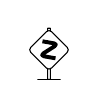
\begin{tikzpicture}[baseline=(x.base)]
		\draw[rounded corners=.01em] (-.05em,-1.07em)rectangle(.05em,.78em);
		\draw[fill=white,rounded corners=1.3] (0,.75em)--(.75em,0)--(0,-.75em)--(-.75em,0)--cycle;
		\draw[line width=0.2mm, line cap=round](-.4em,-1.07em)--(.4em,-1.07em);
		\node(x) at (0,0em) {};
		% Thank you https://tex.stackexchange.com/a/262510
		\draw[
			line cap=but,
			line join=round,
			x=.5em,
			line width=0.5mm,
			y=1*(height("Z")-\pgflinewidth)*(1-sin(10)),
			rotate=-10,
			rounded corners=1.5pt,
		](-0.57, 0.57) -- (0.57, 0.57) -- (-0.57, -0.57) -- (0.57, -0.57);
	\end{tikzpicture}%
}

%%%%%%%%%%%%%%%%%%%%%%%%%%%%%%%%%%%%%%%%%%%% MARGINS
\usepackage{marginnote}
% Thank you https://tex.stackexchange.com/a/472882
% Makes marginnotes always appear on the left, apparently
%
\makeatletter
\long\def\@mn@@@marginnote[#1]#2[#3]{%
	\begingroup
		\ifmmode\mn@strut\let\@tempa\mn@vadjust\else
			\if@inlabel\leavevmode\fi
			\ifhmode\mn@strut\let\@tempa\mn@vadjust\else\let\@tempa\mn@vlap\fi
		\fi
		\@tempa{%
			\vbox to\z@{%
				\vss
				\@mn@margintest
				\if@reversemargin\if@tempswa
						\@tempswafalse
					\else
						\@tempswatrue
				\fi\fi

					\llap{%
						\vbox to\z@{\kern\marginnotevadjust\kern #3
							\vbox to\z@{%
								\hsize\marginparwidth
								\linewidth\hsize
								\kern-\parskip
								%\mn@parboxrestore
								\marginfont\raggedleftmarginnote\strut\hspace{\z@}%
								\ignorespaces#1\endgraf
								\vss
							}%
							\vss
						}%
						\if@mn@verbose
							\PackageInfo{marginnote}{xpos seems to be \@mn@currxpos}%
						\fi
						\begingroup
							\ifx\@mn@currxpos\relax\else\ifx\@mn@currpos\@empty\else
									\kern\@mn@currxpos
							\fi\fi
							\ifx\@mn@currpage\relax
								\let\@mn@currpage\@ne
							\fi
							\if@twoside\ifodd\@mn@currpage\relax
									\kern-\oddsidemargin
								\else
									\kern-\evensidemargin
								\fi
							\else
								\kern-\oddsidemargin
							\fi
							\kern-1in
						\endgroup
						\kern\marginparsep
					}%
			}%
		}%
	\endgroup
}
\makeatother
%
% Mostly for todonotes
\renewcommand{\marginpar}{\marginnote}
%%%%%%%%%%%%%%%%%%%%%%%%%%%%%%%%%%%%%%%%%%%% /MARGINS

\definecolor{nirlightred}{RGB}{250, 220, 220}
\definecolor{nirdarkred}{HTML}{f40000}
\declaretheoremstyle[
	mdframed={
		backgroundcolor=nirlightred,
		linecolor=nirdarkred,
		rightline=false,
		topline=false,
		bottomline=false,
		linewidth=2pt,
		innertopmargin=5pt,
		innerbottommargin=8pt,
		innerleftmargin=8pt,
		leftmargin=-2pt,
		skipbelow=2pt,
		nobreak
	},
	headfont=\normalfont\bfseries\color{nirdarkred}
]{nirredbox}

\makeatletter
\declaretheorem[
	style=nirredbox,
	name=Warning,
	sibling=thm,
	% without \leavevmode, the first item in a list gets misformatted
	postheadhook={\leavevmode\marginnote{\nirwarnsymbol}[-3pt]%
	\ifthmt@thisistheone% restatable makes alignment weird
		\hspace{-2.2pt}%
	\fi}
]{warn}
\makeatother

\title{Algebra I Midterm Review}
\date{\today}
\author{Hui Sun}


\begin{document}

\maketitle

\newpage
\tableofcontents

\chapter{Definitions}
\setcounter{chapter}{1}


\section{Chapter IV: Groups II}
We first recall some definitions.
\begin{defn}[stabilizer, fixed points]
    Let $G$ act on a set $S$, then for $a\in S$, the stabilizer of $Stab_G(a)$ is 
    \begin{equation*}
        Stab_G(a)=\{g\in G: g\cdot a=a\}
    \end{equation*}
    (we use $\cdot$ to denote the action.) And the set of fixed points of this action is 
    \begin{equation*}
        Z=\{a\in S: g\cdot a=a, \text{ for all } g\in G\}
    \end{equation*}
\end{defn}
\begin{prop}
    Let $S$ be a finite set, and let $G$ act on $S$, then 
    \begin{equation*}
        |S|=|Z|+\sum_{a\in A}[G:Stab_G(a)]
    \end{equation*}
    where $A$ has exactly one element from each nontrivial orbit of the action.
\end{prop}
\begin{defn}[$p$-group]
    A $p$-group is a finite group whose order is a power of a prime integer $p$.
\end{defn}
\begin{cor}
    Let $G$ be a $p$-group acting on a finite set $S$, and let $Z$ be the fixed point of the action, then 
    \begin{equation*}
    |Z|\equiv |S|\mod p
    \end{equation*}
    ($[G:Stab_G(a)]$ divides $|G|$.)
\end{cor}
Next we focus on the group action being conjugation.
\begin{defn}[center]
    The center is as follows
    \begin{equation*}
        Z(G)=\{g\in G: ga=ag, \forall a\in G\}
    \end{equation*}
    In other words, the center consists of elemenets that commute with every other element in the group.
\end{defn}
\begin{lem}
    Let $G$ be a finite group, and assume $G/Z(G)$ is cyclic, then $G$ is commutative.
\end{lem}

\begin{defn}[centralizer]
    The centralizer $Z_G(a)$ for $a\in G$ is the stabilizer under conjugation, i.e., 
    \begin{equation*}
        Z_G(a)=\{g\in G: gag^{-1}=a\}=\{g\in G: ga=ag\}
    \end{equation*}
    is the set of elements in $G$ that commute with the given $a$.

    We note that the center $Z(G)=\bigcap_{a\in G}Z_G(a)$.
\end{defn}
\begin{defn}[conjugacy class]
    The conjugacy class of $a\in G$ is the orbit $[a]$ under the conjugation action. And $a,b\in G$ are conjugate if they belong to the same conjugacy class.
\end{defn}
\begin{prop}[class formula]
    Let $G$ be a finite group, then 
    \begin{equation*}
        |G|=|Z(G)|=\sum_{a\in A}[G:Z_G(a)]
    \end{equation*}
    where $A$ is a set containing one representative for each nontrivial conjugacy class in $G$.
\end{prop}
\begin{cor}
    Let $G$ be a nontrivial $p$ group, then $G$ has a nontrivial center.
\end{cor}
Next we talk about conjugation of subsets and subgroups.
\begin{defn}[normalizer, centralizer]
    Let $A\subset G$ be a subset, then $N_G(A)$ is the normalizer of a subset $A$ is $Stab_G(A)$ under conjugation, i.e., 
    \begin{equation*}
        N_G(A)=\{g\in G: gAg^{-1}=A\}
    \end{equation*}
    The centralizer of $A$, $Z_G(A)$ is 
    \begin{equation*}
        Z_G(A)=\{g\in G: gag^{-1}=a, \text{ for all } a\in A\}
    \end{equation*}
    i.e., $Z_G(A)=\bigcap_{a\in A}Z_G(a)$. We note that $Z_G(A)\subset N_G(A)$.

    We interpret $N_G(H)$ as the largest subgroup of $G$ in which $H$ is normal.
\end{defn}
The definition implies that if $H$ is a normal subgroup of $G$, then $N_G(H)=G$.

\begin{lem}
    Let $H\subset G$ be a subgroup, then if finite, then the number of subgroups conjugate to $H$ is equal to the index $[G:N_G(H)]$ of the normalizer $H$ in $G$.
\end{lem}
\begin{prop}
    If $[G:H]$ is finite, then the number of subgroups conjugate to $H$ is finite and divides $[G:H]$.
\end{prop}

Next we begin Sylow theorems.

\begin{prop}[Cauchy's theorem]
    Let $G$ be a finite group, and let $p$ be a prime divisor of $|G|$, then $G$ contains an element of order $p$.
\end{prop}
\begin{cor}
    Let $G$ be a finite grou, and let $p$ be a prime divisor of $|G|$, and let $N$ be the number of cyclic subgroups of $G$ of order $p$, then $N\equiv 1\mod p$.
\end{cor}

\begin{defn}[simple group]
    A group is simple if it is nontrivial and is only normal subgroups are $\{e\}$ and $G$ itself.
\end{defn}

\begin{defn}[$p$-Sylow subgroup]
    Let $p$ be a prime integer, A $p$-Sylow subgroup of a finite group $G$ is a subgroup of order $p^r$, where $|G|=p^rm$ and $\gcd(p,m)=1$. 
\end{defn}
\begin{thm}[Sylow I]
    Every finite group contains a $p$-Sylow subgroup, for all primes $p$.
\end{thm}
The next proposition is stronger and implies Sylow I.
\begin{prop}
    If $p^k$ divides the order of $G$, then $G$ has a subgroup of order $p^k$.
\end{prop}
The second Sylow theorem states that every maximal $p$-group in $|G|$ is a $p$-Sylow subgroup. It is as large as is allowed by Lagrange's.

\begin{thm}[Sylow II]
    Let $G$ be a finite group, let $P$ be a $p$-Sylow subgroup, and $H\subset G$ be a $p$-subgroup, then $H$ is contained in some conjugate of $P$: there exists $g\in G$ such that 
    \begin{equation*}
        H\subset gPg^{-1}
    \end{equation*}
\end{thm}
\begin{prop}
    Let $H$ be a $p$-subgroup of a finite group $G$, assume that $H$ is not a $p$-Sylow subgroup, then there exists a $p$-subgroup $H'$ of $G$ containing $H$, such that 
    \begin{equation*}
        [H':H]=p
    \end{equation*}
    and $H$ is normal in $H'$.
\end{prop}
Here comes the last Sylow theorem.
\begin{thm}[Sylow III]
    Let $p$ be prime, and let $G$ be a finite group of order $|G|=p^rm$, assume $p$ does not divide $m$, then the number of $p$-Sylow subgroups of $G$ divides $m$ and is congruent to $1$ modulo $p$.
\end{thm}
Next we list some applications of Sylow theorems.
\begin{prop}
    Let $G$ be a group of order $mp^r$, where $p$ is a prime integer and $1<m<p$. Then $G$ is not simple.
\end{prop}
\begin{cor}
    Assume $p<q$ are prime integers, and $q\not\equiv 1\mod p$, let $G$ be a group of order $pq$, then $G$ is cycic.
\end{cor}
\begin{cor}
    Let $q$ be an odd prime, and let $G$ be a noncommutative group of order $q$, then $G\cong D_{2q}$, the dihedral group.
\end{cor}

Next we begin composition series and solvability.
\begin{defn}[series]
    A series of subgroups $G_i$ of a group $G$ is a decreasing sequence of subgroups starting from $G$:
    \begin{equation*}
        G=G_0\supsetneq G_1\supsetneq G_2\supsetneq\dots
    \end{equation*}
    where each $\supsetneq$ is strict inclusion.

    The series is normal if $G_{i+1}$ is normal in $G_i$ for all $i$. The maximal length of a normal series is denoted as $l(G)$.
\end{defn}
We note that $l(G)=1$ if and only if $G$ is simple.
\begin{defn}[composition series]
    A composition series for $G$ is a normal series 
    \begin{equation*}
        G=G_0\supsetneq G_1\supsetneq G_2\supsetneq\dots
    \end{equation*}
    such that the successive quotients $G_i/G_{i+1}$ are simple.
\end{defn}

\begin{thm}[Jordan-Holder]
    Let $G$ be a group, and let 
    \begin{equation*}
        G=G_0\supsetneq G_1\supsetneq\dots\supsetneq G_n=\{e\}
    \end{equation*}
    and 
    \begin{equation*}
        G=G_0'\supsetneq G_1'\supsetneq\dots\supsetneq G_n'=\{e\}
    \end{equation*}
    be two composition series for $G$. Then $m=n$ and the lists of quotients groups $H_i=G_i/G_{i+1}$, $H_i'=G_i'/G_{i+1}'$ agree (up to isomorphism) after a permutation of the indices.
\end{thm}
\begin{prop}
    Let $G$ be a group, and let $N$ be a normal subgroup of $G$. Then $G$ has a composition series if and only if both $N$ and $G/N$ have composition series. Further, if this is the case, then 
    \begin{equation*}
        l(G)=l(N)+l(G/N)
    \end{equation*}
    and the composition factors of $G$ consist of the collection of composition factors from $N$ and $G/N$.
\end{prop}
\begin{defn}[refinement]
    A series is a refinement of another series if all terms of the first appear in the second.
\end{defn}
\begin{prop}
    Any two normal series of a finite group ending with $\{e\}$ admit equivalent refinements.

    (The idea is to first refine it to composition series then apply Jordan-Holder).
\end{prop}

\begin{defn}[commutator subgroup]
    Let $G$ be a group, the commutator subgroup of $G$ is the subgroup \textbf{generated} by all elements 
    \begin{equation*}
        [g,h]=ghg^{-1}h^{-1}
    \end{equation*}
    where $g,h\in G$. We denote the commutator subgroup as $[G,G]$.
\end{defn}
\begin{lem}
    Let $\varphi:G\to H$ be a homomorphism, then 
    \begin{equation*}
        \varphi[g,h]=[\varphi(g),\varphi(h)]
    \end{equation*}
\end{lem}
\begin{prop}
    Let $[G,G]$ be commutator subgroup of $G$, then 
    \begin{enumerate}
        \item $[G,G]$ is normal in $G$.
        \item The quotient $G/[G,G]$ is commutative.
        \item If $\alpha: G\to A$ is a homomorphism to some commutative group $A$, then 
        \begin{equation*}
            [G,G]\subset\ker\alpha
        \end{equation*}
        \item the natural projection $G\to G/[G,G]$ is universal in the category of homomorphisms $\alpha:G\to A$ where $A$ is some commutative group.
    \end{enumerate}
\end{prop}
One can get taking the commutator:
\begin{defn}[derived series]
    Let a derived series of $G$ be as follows:
    \begin{equation*}
        G\supset [G,G]\supset [[G,G], [G,G]]\supset\dots
    \end{equation*}
\end{defn}
\begin{defn}[solvable]
    A group is solvable if its derived series terminates with the identity.
\end{defn}
\begin{prop}
    For a finite group $G$, then the following are equivalent:
    \begin{enumerate}
        \item $G$ is solvable.
        \item All composition factors of $G$ are cycic.
        \item $G$ admits a cyclic series ending in $\{e\}$.
        \item $G$ admits an abelian series ending in $\{e\}$.
    \end{enumerate}
\end{prop}
\begin{cor}
    All $p$-groups are solvable.
\end{cor}
\begin{cor}
    Let $N$ be a normal subgroup of a group $G$, then $G$ is solvable if and only if both $N, G/N$ are solvable.
\end{cor}
Next we talk about symmetric group.
\begin{defn}[cycle]
    A nontrivial cycli is an element of $S_n$ with exactly one nontrivial orbit. For distinct $a_1, \dots, a_r$ in $\{1,\dots,n\}$, the notation 
    \begin{equation*}
        (a_1a_2\dots a_n)
    \end{equation*}
    denote the cycle in $S_n$ with nontrivial orbit $\{a_1,\dots, a_r\}$, acting as 
    \begin{equation*}
        a_1\mapsto a_2\mapsto a_2\mapsto \dots a_r\mapsto a_1
    \end{equation*}
    In this case, $r$ is the lenght of the cycle. A cycle of length $r$ is called an $r$-cycle.
\end{defn}
\begin{lem}
    Disjoint cycles commute.
\end{lem}
\begin{lem}
    For every $\sigma\in S_n$, where $\sigma\neq e$, can be written as a product of disjoint nontrivial cycles, in a unique way up to permutations of the factors.
\end{lem}

\begin{defn}[type]
    The type of $\sigma\in S_n$ is the parittion of $n$ given by the size of the orbits of the action of $\la \sigma\ra$ on $\{1,\dots,n\}$.

    For example, $\sigma=(18632)(47)(5)$ has type $[5,2,1]$.
\end{defn}
\begin{lem}
    Let $\tau\in S_n$, and let $(a_1\dots a_r)$ be a cycle, then 
    \begin{equation*}
        \tau(a_1\dots a_r)\tau^{-1}=(\tau^{-1}a_1\dots\tau^{-1}(a_n))
    \end{equation*}
\end{lem}
\begin{prop}
    Two elements of $S_n$ are conjugate in $S_n$ if and only if they have the same type.
\end{prop}

\begin{cor}
    The number of conjugacy classes in $S_n$ equals the number of parititons of $n$.
\end{cor}
Next we talk about alternating groups.
\begin{defn}[sign]
    The sign of a permutation $\sigma\in S_n$, denoted as $(-1)^\sigma$, is determined by the action of $\sigma$ on $\Delta_n$, where 
    \begin{equation*}
        \Delta_n=\prod_{1\leq i<j\leq n}(x_i-x_j)
    \end{equation*}
    which is in $\mathbb{Z}[x_1,\dots,x_n]$, and 
    \begin{equation*}
        \Delta_n\sigma=\prod_{1\leq i<j\leq n}(x_{\sigma(i)}-x_{\sigma(j)})
    \end{equation*}
    and 
    \begin{equation*}
        \Delta_n\sigma=(-1)^\sigma\Delta_n
    \end{equation*}
\end{defn}
\begin{lem}
    Transpositions generate $S_n$.
\end{lem}
\begin{lem}
    Let $\sigma=\tau_1\dots\tau_r$ be a product of transpositions, then $\sigma$ is even when $r$ is even, and odd when $r$ is odd.
\end{lem}
\begin{defn}[alternating group]
    The alternating group on $\{1,\dots,n\}$, denoted $A_n$, consists of even permutations $\sigma\in S_n$. 

    We note that $A_n$ is a normal subgroup of $S_n$, and $[S_n:A_n]=2$.
\end{defn}
Next we talk about conjugacy class of $A_n$, solvability of $S_n$, etc.
\begin{lem}
    Let $n\geq 2$, and $\sigma\in A_n$, then 
    \begin{equation*}
        [\sigma]_{A_n}=[\sigma]_{S_n}
    \end{equation*}
    or the size of $[\sigma]_{A_n}$ is half hte size of $[\sigma]_{S_n}$, according to whether the centralizer $Z_{S_n}(\sigma)$ is not or is contained in $A_n$.
\end{lem}
\begin{prop}
    Let $\sigma\in A_n$, where $n\geq 2$, then the conjugacy class of $\sigma$ in $S_n$ splits into two conjugacy classes in $A_n$ precisely if the type of $\sigma$ consists of distinct odd numbers.
\end{prop}
\begin{cor}
    The alternating group $A_5$ is a simple noncommutative group of order 60.
\end{cor}
\begin{lem}
    The alternating group $A_n$ is generated by 3-cycles.
\end{lem}
\begin{prop}
    Let $n\geq 5$, if a normal subgroup of $A_n$ contains a 3-cycle, then it contains all 3-cycles.
\end{prop}
\begin{thm}
    The alternating group $A_n$ is simple for all $n\geq 5$.
\end{thm}
\begin{cor}
    For $n\geq 5$, the group $S_n$ is not solvable.
\end{cor}

Next we talk about products of groups.

\begin{lem}
    Let $N,H$ be normal subgroups of a group $G$, then 
    \begin{equation*}
        [N,H]\subset N\cap H
    \end{equation*}
\end{lem}
\begin{cor}
    Let $N,H$ be normal subgroups of a group $G$, assume $N\cap H=\{e\}$, then $N,H$ commute, i.e., for all $n\in N, h\in H$, we have 
    \begin{equation*}
        nh=hn
    \end{equation*}
\end{cor}
\begin{prop}
    Let $N,H$ be normal subgroups, and $N\cap H=\{e\}$, then 
    \begin{equation*}
        NH\cong N\times H
    \end{equation*}
\end{prop}
Next we talk about groups in exact sequences.
\begin{defn}[extension]
    Let $N,H$ be groups, a group $G$ is an extension of $H$ by $N$ if there is an exact sequence of groups:
    \begin{equation*}
        1\to N\to G\to H\to 1
    \end{equation*}
\end{defn}
\begin{defn}[split]
    An exact sequence of groups is said to split if $H$ may be identified with a subgroup of $G$, so that 
    \begin{equation*}
        N\cap H=\{e\}
    \end{equation*}
\end{defn}
\begin{lem}
    Let $N$ be a normal subgroup of a group $G$, and let $H$ be a subgroup of $G$ such that $G=NH$ and $N\cap H=\{e\}$. Then $G$ is a split extension of $H$ by $N$.
\end{lem}
Next we define internal and semidirect products.
\begin{defn}
    Let $N,H$ be any two groups and an arbitrary homomorphism
    \begin{equation*}
        \theta:H\to Aut(N), h\mapsto\theta_h
    \end{equation*}
    define an operation $\bullet_\theta$ on the set $N\times H$ as follows: for $n_1, n_2\in N, h_1,h_2\in H$, we have 
    \begin{equation*}
        (n_1,h_1)\bullet_\theta(n_2,h_2)=(n_1\theta_{h_1}(n_2), h_1h_2)
    \end{equation*}
\end{defn}
\begin{lem}
    The resulting structure $(N\times H, \bullet_\theta)$ is a group, with the identity element $(e_N, e_H)$.
\end{lem}
\begin{defn}
    The group $(N\times H, \bullet_\theta)$ is a semidirect product of $N,H$ and is denoted by $N\rtimes_\theta H$.
\end{defn}
\begin{prop}
    Let $N,H$ be groups, and let $\theta:H\to Aut(N)$ be a homomorphism, let $G=N\rtimes_\theta H$ be the corresponding semidirect product. Then 
    \begin{enumerate}
        \item $G$ contains isomorphic copies of $N$ and $H$.
        \item The natrual projection $G\to H$ is a surjective homomorphism, with kernel $N$, thus $N$ is normal in $G$, and the sequence 
        \begin{equation*}
            1\to N\to N\rtimes_\theta H\to H\to 1
        \end{equation*}
        is split exact.
        \item $N\cap H=\{e_G\}$.
        \item $G=NH$.
        \item The homomorphism $\theta$ is realized by conjugation in $G$: that is, for $h\in H$ and $n\in N$, we have
        \begin{equation*}
            \theta_h(n)=hnh^{-1}
        \end{equation*}
        in $G$.
    \end{enumerate}
\end{prop}
\begin{prop}
    Let $N,H$ be subgroups of a group $G$, with $N$ normal in $G$. Assume that $N\cap H=\{e\}$, and $G=NH$, let $\gamma:H\to Aut(N)$ be defined by conjugation: for $h\in H, n\in N$, we have 
    \begin{equation*}
        \gamma_h(n)=hnh^{-1}
    \end{equation*}
    then 
    \begin{equation*}
        G\cong N\rtimes_\gamma H
    \end{equation*}
\end{prop}
We now talk about finite abelian groups.
\begin{lem}
    Let $G$ be commutative, and let $H,K$ be subgroups such that $|H|,|K|$ are relatively prime, then 
    \begin{equation*}
        H+K\cong H\oplus K
    \end{equation*}
\end{lem}
\begin{cor}
    Every finite abelian group is the direct sum of its nontrivial Sylow subgroups.
\end{cor}
\begin{lem}
    Let $G$ be a commutative $p$-group, and let $g\in G$ be an element of maximal order, then the exact sequence 
    \begin{equation*}
        0\to \la g\ra\to G\to G/\la g\ra\to 0
    \end{equation*}
    splits.
\end{lem}
\begin{lem}
    Let $p$ be a prime integer and $r\geq 1$, let $G$ be a noncyclic abelian group of order $p^{r+1}$, and let $g\in G$ be an element of order $p^r$. Then there exists an element $h\in G$, where $h\not\in\la g\ra$, such that 
    \begin{equation*}
        |h|=p
    \end{equation*}
\end{lem}
\begin{cor}
    Let $G$ be a finite abelian groups, then $G$ is a direct sum of cyclic $p$-groups.
\end{cor}
\begin{thm}
    Let $G$ be a finite nontrivial commutative group, then 
    \begin{enumerate}
        \item There exist prime integers $p_1,\dots, p_r$ and positive integers $n_{ij}$ such that $|G|=\prod_{i,j}p_i^{n_{i,j}}$ and 
        \begin{equation*}
            G\cong\bigoplus_{i,j}\frac{\mathbb{Z}}{p_i^{n_{i,j}}\mathbb{Z}}
        \end{equation*}
        \item There exist positive integers $1<d_1\vert\dots\vert d_s$ such that $|G|=d_1\dots d_s$ and 
        \begin{equation*}
            G\cong \frac{\Z}{d_1\Z}\oplus\dots\oplus\frac{\Z}{d_s\Z}
        \end{equation*}
    \end{enumerate}
\end{thm}
\begin{lem}
    Let $G$ be a finite abelian group, and assume that for every integer $n>0$, the number of elements $g\in G$ such that $ng=0$ is at most $n$. Then $G$ is cyclic.
\end{lem}

\begin{thm}
    Let $F$ be a field, and let $G$ be a finite subgroup of the multiplicative group $(F^*,\cdot)$, then $G$ is cyclic.
\end{thm}











\end{document}